\section{Рабочий проект}
\subsection{Описание классов системы}
Система реализована с помощью следующих программных классов:

\begin{itemize}
	\item \textquotedbl main \textquotedbl является фундаментальным классом для главного меню. Помимо основных свойств, таких как connection, экземпляров utils, controller и tables, содержит в себе стартовые виджеты;
	\item \textquotedbl Controller \textquotedbl -- расширяет \textquotedbl main \textquotedbl, представляя панель управления таблицами, необходимую для взаимодействия пользователя с данными внутри таблицы;
	\item \textquotedbl Utils \textquotedbl применяется для отправки запросов в БД. Содержит только самые необходимые методы, взаимодействующие с БД непосредственно;
	\item \textquotedbl Tables \textquotedbl служит для формирования необходимых сложных запросов к БД. Сформировав строку, класс использует \textquotedbl Utils \textquotedbl для отправки;
	\item \textquotedbl Validator \textquotedbl представляет собой служебный класс, конфигурирующий интерфейс таким образом, чтобы пользователь не мог ввести данные неподходящего формата.
\end{itemize}

Описание полей и методов программных классов приведено в таблицах \ref{class:table1}-\ref{class:table5}.

\renewcommand{\arraystretch}{0.8} % уменьшение расстояний до сетки таблицы
\begin{xltabular}{\textwidth}{|X|p{2.5cm}|>{\setlength{\baselineskip}{0.7\baselineskip}}p{4.85cm}|>{\setlength{\baselineskip}{0.7\baselineskip}}p{4.85cm}|}
\caption{Описание класса main\label{class:table1}}\\
\hline \centrow \setlength{\baselineskip}{0.7\baselineskip} Название класса & \centrow \setlength{\baselineskip}{0.7\baselineskip} Модуль, к которому относится класс & \centrow Описание поля/метода & \centrow Поле/метод \\
\hline \centrow 1 & \centrow 2 & \centrow 3 & \centrow 4\\ \hline
\endfirsthead
\continuecaption{Продолжение таблицы \ref{class:table1}}
\centrow 1 & \centrow 2 & \centrow 3 & \centrow 4\\ \hline
\finishhead
main & Главный модуль & isES -- поле для определения режима работы программы (Обычный или ЧС) & bool isES\\
\hline  & Главный модуль & window -- экземпляр класса customtkinter.CTk(), представляющий окно & CTk window\\
\hline  & Главный модуль & frame -- экземпляр класса customtkinter.CTkFrame(), представляющий поле для виджетов & CTkFrame frame\\
\hline  & Главный модуль & connection -- строка, содержащая путь для подключения к БД & string connection\\
\hline  & Главный модуль & ask\underline{ }lb, timer\underline{ }lb -- виджеты текста в главном меню &
CTkLabel ask\underline{ }lb

CTkLabel timer\underline{ }lb
\\
\hline  & Главный модуль & pns\underline{ }btn, rms\underline{ }btn, drs\underline{ }btn, psr\underline{ }btn, psr\underline{ }ua\underline{ }btn -- виджеты кнопок в главном меню &
CTkButton pns\underline{ }btn

CTkButton rms\underline{ }btn

CTkButton drs\underline{ }btn

CTkButton psr\underline{ }btn

CTkButton psr\underline{ }ua\underline{ }btn
\\
\hline  & Главный модуль & on\underline{ }closing -- метод для вывода вопроса о том, уверен ли пользователь в своём решении выйти & on\underline{ }closing() Возвращает: ничего\\ 
\end{xltabular}
\renewcommand{\arraystretch}{1.0} % восстановление сетки
 
\begin{xltabular}{\textwidth}{|X|p{2.5cm}|>{\setlength{\baselineskip}{0.7\baselineskip}}p{4.85cm}|>{\setlength{\baselineskip}{0.7\baselineskip}}p{4.85cm}|}
	\caption{Описание класса Controller \label{class:table2}}\\
	\hline \centrow \setlength{\baselineskip}{0.7\baselineskip} Название класса & \centrow \setlength{\baselineskip}{0.7\baselineskip} Модуль, к которому относится класс & \centrow Описание поля/метода & \centrow Поле/метод \\
	\hline \centrow 1 & \centrow 2 & \centrow 3 & \centrow 4\\ \hline
	\endfirsthead
	\continuecaption{Продолжение таблицы \ref{class:table2}}
	\centrow 1 & \centrow 2 & \centrow 3 & \centrow 4\\ \hline
	\finishhead
Controller & Главный модуль & styles\underline{ }init -- метод для инициализации стилей и добавления его в список ttk.element\underline{ }names & styles\underline{ }init(st). Принимает на вход экземпляр класса Style, который будет настраивать. 

Возвращает: ничего\\
\hline  & Главный модуль & show\underline{ }table -- метод для перехода к панели управления выбранной таблицей. Отображает, настраивает и группирует каждый элемент по сетке & show\underline{ }table(which, window, tables, connection). 

Принимает на вход название таблицы, экземпляр окна, экземпляр tables, и строку подключения connection. 

Возвращает: ничего\\
\hline  & Главный модуль & fields\underline{ }creation -- метод, вызываемый в show\underline{ }table и дополняющий его. Определяет и направленно настраивает поля ввода информации & fields\underline{ }creation(which, frameEx, window). 

На вход принимает название таблицы, экземпляр поля для виджетов, экземпляр окна.

Возвращает: tuple (validatedTFs, combolist) -- кортеж сформированных полей ввода\\
\hline  & Главный модуль & clear -- метод, очищающий поля ввода & clear(keyLabel, combinedControls, window). 

На вход принимает таблицу отображения Id текущей строки для очищения, кортеж полей ввода, экземпляр окна. 

Возвращает: ничего\\
\hline  & Главный модуль & TreeCreate -- метод, отображающий текущую таблицу в виде виджета древа & TreeCreate(tree, table, tableWin, connection). 

На вход принимает экземпляр класса ttk.TreeView, который будет пересоздавать, название таблицы, экземпляр поля виджетов, строку подключения. 

Возвращает: TreeView.tree -- созданный виджет древа\\
\hline  & Главный модуль & TreeRefresh -- метод, обновляющий виджет древа & TreeRefresh(tree, table, connection). 

На вход принимает экземпляр класса ttk.TreeView, который будет обновлять, название таблицы, строку подключения. 

Возвращает: Ничего\\
\hline  & Главный модуль & MoveTo -- метод для перехода просмотра к конкретному элементу таблицы по индентификатору & MoveTo(id, table, combinedControls, currentLb, window, connection). 

На вход принимает идентификатор элемента для перехода, имя таблицы, кортеж полей вывода, табличку отображения текущего Id, экземпляр окна и строку подключения. 

Возвращает: Ничего\\
\hline  & Главный модуль & show\underline{ }acc -- метод для перехода к окну проверки доступа & show\underline{ }acc(connection, isES, tables, window). 

На вход принимает строку подключения к БД, флаг ЧС, экземпляр класса tables, экземпляр окна. 

Возвращает: Ничего\\
\hline  & Главный модуль & toggle\underline{ }ES -- метод обработки состояний переключателя, применяемый в определении одной из двух таблиц для показа & toggle\underline{ }ES(switch, psrlb, tables,connection, tree, isES). 

На вход принимает экземпляр переключателя, текстовое поле для изменения выводимой информации, строку подключения, экземпляр виджета древа и флаг ЧС.

\end{xltabular}

\renewcommand{\arraystretch}{1.0} % восстановление сетки

\begin{xltabular}{\textwidth}{|X|p{2.5cm}|>{\setlength{\baselineskip}{0.7\baselineskip}}p{4.85cm}|>{\setlength{\baselineskip}{0.7\baselineskip}}p{4.85cm}|}
	\caption{Описание класса Utils \label{class:table3}}\\
	\hline \centrow \setlength{\baselineskip}{0.7\baselineskip} Название класса & \centrow \setlength{\baselineskip}{0.7\baselineskip} Модуль, к которому относится класс & \centrow Описание поля/метода & \centrow Поле/метод \\
	\hline \centrow 1 & \centrow 2 & \centrow 3 & \centrow 4\\ \hline
	\endfirsthead
	\continuecaption{Продолжение таблицы \ref{class:table3}}
	\centrow 1 & \centrow 2 & \centrow 3 & \centrow 4\\ \hline
	\finishhead
Utils & Главный модуль & create\underline{ }connection -- метод создаёт подключение к базе данных & create\underline{ }connection(path). 

На вход принимает строковый путь к файлу базы данных. 

Возвращает: sqlite3.connection connection - экземпляр созданного подключения\\
\hline  & Главный модуль & read\underline{ }single\underline{ }row -- считывает единственную строку с БД & read\underline{ }single\underline{ }row(id, connection, table). 

На вход принимает идентификатор, по которому будет считываться строка, экземпляр подключения, название таблицы 

Возвращает: строку в формате кортежа\\
\hline  & Главный модуль & execute\underline{ }query -- посылает команду в БД & execute\underline{ }query(
connection, query).

На вход принимает экземпляр подключения и строку команды для выполнения.

Возвращает: bool True/bool False -- флаг о том, успешно ли выполнен запрос\\
\hline  & Главный модуль & execute\underline{ }read\underline{ }query -- отдельный метод для послания запроса в БД на чтение & execute\underline{ }read\underline{ }query(
connection, query).

На вход принимает экземпляр подключения и строку команды для выполнения.

Возвращает: строку в формате кортежа\\
\hline  & Главный модуль & timetick -- асинхронный метод для отображения и вывода текущего времени в главном меню & timetick(timerLb).

На вход принимает, куда будет выводиться время.

Возвращает: ничего\\
\hline  & Главный модуль & asyncMLoop -- метод для обеспечения асинхронной работы окна с часами & asyncMLoop(wndw).

На вход принимает окно главного меню.

Возвращает: ничего\\
\hline  & Главный модуль & asyncStart -- асинхронный метод для настройки взаимодействия главного меню с часами в асинхронном порядке и обновления полей со временем в БД & asyncStart(window, timer\underline{ }lb, connection).

На вход принимает экземпляр окна, поле для вывода времени, строку подключения к БД.

Возвращает: Ничего\\
	
\end{xltabular}
\renewcommand{\arraystretch}{1.0} % восстановление сетки

\begin{xltabular}{\textwidth}{|X|p{2.5cm}|>{\setlength{\baselineskip}{0.7\baselineskip}}p{4.85cm}|>{\setlength{\baselineskip}{0.7\baselineskip}}p{4.85cm}|}
	\caption{Описание класса Tables \label{class:table4}}\\
	\hline \centrow \setlength{\baselineskip}{0.7\baselineskip} Название класса & \centrow \setlength{\baselineskip}{0.7\baselineskip} Модуль, к которому относится класс & \centrow Описание поля/метода & \centrow Поле/метод \\
	\hline \centrow 1 & \centrow 2 & \centrow 3 & \centrow 4\\ \hline
	\endfirsthead
	\continuecaption{Продолжение таблицы \ref{class:table4}}
	\centrow 1 & \centrow 2 & \centrow 3 & \centrow 4\\ \hline
	\finishhead
	Tables & Главный модуль & self\underline{ }definition -- метод переводит названия таблиц данных с русского языка на английский для последующих запросов к БД & self\underline{ }definition(which). 
	
	На вход принимает строку названия на русском языке. 
	
	Возвращает: строку названия на английском языке\\
	\hline  & Главный модуль & timeAppend -- метод, переводящий строку времени из формата <<ЧЧММСС>> в формат <<ЧЧ:ММ:СС>> & timeAppend(timeString). 
	
	На вход принимает неотформатированную строку времени. 
	
	Возвращает: строку времени в отформатированном виде\\
	\hline  & Главный модуль & penalty\underline{ }check -- метод, сравнивающий данные о штрафных ограничениях данных о Дверях и данных о Штрафах & penalty\underline{ }check(pennies, type). 
	
	На вход принимает кортеж из найденных по принадлежности штрафов и строку типа штрафа, с которой нужно сопоставить элементы кортежа. 
	
	Возвращает: флаг о том, совпали ли типы\\
	\hline  & Главный модуль & check\underline{ }access -- метод реализации опции <<Проверка доступа>>, проверяет введённые данные на наличие в базе и выводит информацию о предоставлении доступа. & check\underline{ }access(psr\underline{ }Tf, dor\underline{ }Tf, switch, connection). 
	
	На вход принимает экземпляры текстовых полей куда были введены идентификаторы для поиска, жкземпляр переключателя, строку подключения к БД. 
	
	Возвращает: ничего\\
	\hline  & Главный модуль & start\underline{ }accesses -- метод заполнения данных о доступе пассажиров к дверям по каждому из критериев ограничений. & start\underline{ }accesses(
	connection, psr\underline{ }switch). 
	
	На вход принимает строку подключения к БД и экземпляр переключателя. 
	
	Возвращает: ничего\\
	\hline  & Главный модуль & add\underline{ }element -- метод, реализующий опцию формирования запроса добавления элемента в БД. & add\underline{ }element(table, combinedControls, currentLb, tree, tableWin, connection, window). 
	
	На вход принимает строку названия таблицы, кортеж полей ввода, экземпляр текстового поля для отображения идентификатора текущего элемента, экземпляр виджета древа, экземпляр контейнера для виджетов, строку подключения, экземпляр окна. 
	
	Возвращает: ничего\\
	\hline  & Главный модуль & delete\underline{ }element -- метод, реализующий опцию формирования запроса удаления элемента в БД. & delete\underline{ }element(table, key, currentLb, combinedControls, tree, connection, window). 
	
	На вход принимает строку названия таблицы, идентификатор текущего элемента, кортеж полей ввода, экземпляр текстового поля для отображения идентификатора текущего элемента, экземпляр виджета древа, строку подключения, экземпляр окна. 
	
	Возвращает: ничего\\
	\hline  & Главный модуль & update\underline{ }element -- метод, реализующий опцию формирования запроса изменения элемента в БД. & update\underline{ }element(table, combinedControls, key, tree, connection). 
	
	На вход принимает строку названия таблицы, кортеж полей ввода,  идентификатор текущего элемента, экземпляр виджета древа, строку подключения.
	
	Возвращает: ничего\\
	\hline  & Главный модуль & search\underline{ }element -- метод, реализующий опцию поиска элемента в БД. & search\underline{ }element(
	combinedControls, table, tf, currentLb, connection, window). 
	
	На вход принимает кортеж полей ввода, строку названия таблицы, текстовое поля для воода идентификатора поиска, экземпляр текстового поля для отображения идентификатора текущего элемента,  строку подключения.
	
	Возвращает: ничего\\
	\hline  & Главный модуль & list\underline{ }table -- метод, реализующий опцию \textquotedbl пролистывания \textquotedbl текущей таблицы данных. & list\underline{ }table(direction, table, connection, window). 
	
	На вход принимает флаг направления (вперёд или назад), строку названия таблицы, строку подключения к БД, экземпляр окна.
	
	Возвращает: массив данных текущего элемента\\
	\hline  & Главный модуль & configure\underline{ }list -- метод, дополняющий list\underline{ }table и выводящий данные текущего элемента в поля ввода . & configure\underline{ }list(direction, table, combinedControls, currentLb, connection, window). 
	
	На вход принимает флаг направления (вперёд или назад), строку названия таблицы, кортеж полей ввода, экземпляр текстового поля для отображения идентификатора текущего элемента, строку подключения к БД, экземпляр окна.
	
	Возвращает: массив данных текущего элемента\\
	
\end{xltabular}
\renewcommand{\arraystretch}{1.0} % восстановление сетки


\begin{xltabular}{\textwidth}{|X|p{2.5cm}|>{\setlength{\baselineskip}{0.7\baselineskip}}p{4.85cm}|>{\setlength{\baselineskip}{0.7\baselineskip}}p{4.85cm}|}
	\caption{Описание класса Validator \label{class:table5}}\\
	\hline \centrow \setlength{\baselineskip}{0.7\baselineskip} Название класса & \centrow \setlength{\baselineskip}{0.7\baselineskip} Модуль, к которому относится класс & \centrow Описание поля/метода & \centrow Поле/метод \\
	\hline \centrow 1 & \centrow 2 & \centrow 3 & \centrow 4\\ \hline
	\endfirsthead
	\continuecaption{Продолжение таблицы \ref{class:table5}}
	\centrow 1 & \centrow 2 & \centrow 3 & \centrow 4\\ \hline
	\finishhead
	Validator & Главный модуль & connection -- строка для подключения к базе данных & string connection\\
	\hline  & Главный модуль & validation\underline{ }digits -- метод, использующийся для регистрации правила валидации цифр & validation\underline{ }digits(
	stringVal). 
	
	На вход принимает строку для проверки соответствия правилу.
	
	Возвращает: ту часть строки, что соответствует маске цифр\\
	\hline  & Главный модуль & validation\underline{ }text -- метод, использующийся для регистрации правила валидации символов Кириллицы & validation\underline{ }text(
	stringVal). 
	
	На вход принимает строку для проверки соответствия правилу.
	
	Возвращает: ту часть строки, что соответствует маске символов Кириллицы\\
	\hline  & Главный модуль & validation\underline{ }char -- метод, использующийся для регистрации правила валидации единичного символа Кириллицы & validation\underline{ }char(
	stringVal). 
	
	На вход принимает строку для проверки соответствия правилу.
	
	Возвращает: ту часть строки, что соответствует маске единичного символа Кириллицы\\
	\hline  & Главный модуль & validation\underline{ }time -- метод, использующийся для регистрации правила валидации текстового поля для ввода времени & validation\underline{ }time(
	stringVal). 
	
	На вход принимает строку для проверки соответствия правилу.
	
	Возвращает: ту часть строки, что соответствует маске формата времени\\
	\hline  & Главный модуль & FKValid -- метод, проверяющий наличие элемента с идентификатором для создания внешнего ключа & FKValid(number, tableName). 
	
	На вход принимает номер для поиска, строку названия таблицы.
	
	Возвращает: флаг о том, был ли найден элемент\\
	\hline  & Главный модуль & validate\underline{ }single -- метод, задающий правила ввода для единичного поля ввода & validate\underline{ }single(element, window, type). 
	
	На вход принимает экземпляр поля ввода, экземпляр окна, строку типа валидации.
	
	Возвращает: поле ввода с изменёнными правилами\\
	\hline  & Главный модуль & validate\underline{ }whole -- метод, задающий правила ввода для массива полей ввода & validate\underline{ }whole(tfS, which, window). 
	
	На вход принимает массив полей ввода, строку названия таблицы данных, экземпляр окна.
	
	Возвращает: массив полей ввода с изменёнными правилами\\
	\hline  & Главный модуль & overvalidation -- метод, проверяющий уже введённые данные на корректность перед отправкой & overvalidation(table, combinedControls). 
	
	На вход принимает строку названия таблицы, кортеж полей ввода.
	
	Возвращает: флаг соответствия корректности\\
	
\end{xltabular}
\renewcommand{\arraystretch}{1.0} % восстановление сетки
\subsection{Модульное тестирование программной системы}
\subsubsection{Структура тестового проекта}

В рамках тестирования программного обеспечения была разработан тестовый проект, структура которого представлена на рисунке~\ref{fig:test1}. Данный проект включает в себя модульные тесты для различных компонентов системы.
Тестирование моделей и контроллеров позволяет обеспечить надежность и корректность работы программного обеспечения. 
\begin{figure}[H]
	\centering
	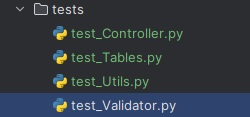
\includegraphics[width=1\linewidth]{images/test1}
	\caption{Структура тестового проекта}
	\label{fig:test1}
\end{figure}
Тестовый проект включает в себя следующие ключевые элементы:
\begin{itemize}
	\item test\underline{ }Controller.py: Наборы модульных тестов для класса панели управления Controller;
	\item test\underline{ }Tables.py: Наборы модульных тестов для класса формирования запросов к БД Tables;
	\item test\underline{ }Validator.py: Наборы модульных тестов для вспомогательного класса валидации Validator;
	\item test\underline{ }Utils.py: Наборы модульных тестов для cлужебного класса запросов в БД.
\end{itemize}
Модульные тесты для класса Tables.py, который является основным классом для формирования запросов в БД, позволяют проверить корректность
логики и поведения этого компонента и исключить возникновение проблем в этом классе. Тесты охватывают такие аспекты, как самоопределение имени раздела данных, а также форматирование строки времени перед запросом.
Модульные тесты класса Tables.py представлены на рисунке \ref{tablestest:image}.

\begin{figure}[H]
\begin{lstlisting}[language=Python]
from Tables import *
import unittest

	class TablesTest(unittest.TestCase):
	def test_self_definition(self):
		self.assertEqual(Tables.self_definition("Пассажиры"), "Passengers")
		self.assertEqual(Tables.self_definition("Двери"), "Doors")
		self.assertEqual(Tables.self_definition("Комнаты"), "Rooms")
		self.assertEqual(Tables.self_definition("Штрафы"), "Penalties")
		self.assertEqual(Tables.self_definition("Дети"), "Passengers_Underage")
		self.assertEqual(Tables.self_definition("Доступы"), "Accesses")
		self.assertEqual(Tables.self_definition("ДоступыЧС"), "Accesses_ES")
	
	def test_invalid_definition(self):
		self.assertEqual(Tables.self_definition("ААААААААААААА"), "Unknown_table")
		self.assertEqual(Tables.self_definition([]), "Invalid table name type")
		self.assertEqual(Tables.self_definition(3), "Invalid table name type")
		self.assertEqual(Tables.self_definition(None), "Invalid table name type")
	
	def test_timeAppend(self):
		self.assertEqual(Tables.timeAppend("200000"), "20:00:00")
		self.assertEqual(Tables.timeAppend("032914"), "03:29:14")
	
	def test_invalid_time(self):
		self.assertEqual(Tables.timeAppend(([2], ['a'])), "Invalid time type")
		self.assertEqual(Tables.timeAppend("14"), "Time format error")
		self.assertEqual(Tables.timeAppend("320000"), "Invalid hours")
		self.assertEqual(Tables.timeAppend("238911"), "Invalid minutes")
		self.assertEqual(Tables.timeAppend("232399"), "Invalid seconds")
		self.assertRaises(ValueError, Tables.timeAppend, "*2****")
	def test_penalty_check(self):
		self.assertEqual(Tables.penalty_check([(1, 'Да', 'Да', 3, 'Загрязнение', 2, '2024-05-15 22:22:09')],"Хулиганство"), True)
		self.assertEqual(Tables.penalty_check([(1, 'Да', 'Нет', 3, 'Загрязнение', 1, '2024-02-15 11:03:12')], "Загрязнение"), False)
	
	def test_wrong_penalty_check(self):
		self.assertEqual(Tables.penalty_check([(1, 2, 3)],"Хулиганство"), "Not a penalty tuple given")
		self.assertEqual(Tables.penalty_check([(1, 'Да', 'Нет', 3, 'Загрязнение', 1, '2024-02-15 11:03:12')], ""), "Wrong penalty type")
		self.assertEqual(Tables.penalty_check([(1, 'Да', 'Нет', 3, 'Загрязнение', 1, '2024-02-15 11:03:12')], "Поведение - неуд"),"Wrong penalty type")

if __name__ == '__main__':
	unittest.main()
%\end{lstlisting}  
\caption{Модульный тест класса Tables.py}
\label{tablestest:image}
\end{figure}

Модульные тесты для класса Utils.py, который является основным классом для отправки запросов в БД, позволяют проверить корректность
логики и поведения базы данных в ответ на запросы этого компонента и исключить возникновение проблем в этом классе. Тесты охватывают такие аспекты, как создание подключения, чтение строки, общий запрос.
Модульные тесты класса Utils.py представлены на рисунке \ref{utilstest:image}.

\begin{figure}[H]
\begin{lstlisting}[language=Python]
import sqlite3
	
from Utils import *
import unittest
	
class UtilsTest(unittest.TestCase):
	def test_create_connection_fail(self):
		self.assertRaises(FileNotFoundError, Utils.create_connection, "")
		self.assertEqual(Utils.create_connection(2),"Wrong path format given")
		self.assertEqual(Utils.create_connection([(1,3), ("Diploma1.db", "someDb.db")]), "Wrong path format given")
	
	def test_execute_read_query(self):
		self.assertEqual(Utils.read_single_row("","",""), "ID should be int natural value")
		self.assertEqual(Utils.read_single_row(1, "", ""), "Wrong table name given")
		self.assertEqual(Utils.read_single_row(1, "", [2]), "Wrong table name given")
		self.assertEqual(Utils.read_single_row(-2, "", ""), "ID should be int natural value")
		#self.assertRaises(KeyError, Utils.read_single_row, -1, sqlite3.connect("Diploma1.db"),"Doors")
	
	def test_execute_invalid_query(self):
		self.assertRaises(SyntaxError,Utils.execute_query,sqlite3.connect("Diploma1.db"), f""" I AM COMMAND""")
		self.assertEqual(Utils.execute_query(sqlite3.connect("Diploma1.db"), ...), "Invalid query given")
	
	def test_execute_right_query(self):
		self.assertEqual(Utils.execute_query(sqlite3.connect("Diploma1.db"), f""" SELECT * FROM Doors"""), True)
		self.assertEqual(Utils.execute_query(sqlite3.connect("Diploma1.db"), f""" SELECT * FROM Rooms WHERE ID>0"""), True)
if __name__ == '__main__':
unittest.main()
		%\end{lstlisting}  
		\caption{Модульный тест класса Utils.py}
		\label{utilstest:image}
\end{figure}

На рисунках ~\ref{fig:test2} - ~\ref{fig:test3} представлены результаты выполнения модульных тестов, подтверждающие успешную проверку всех компонентов системы, что свидетельствует об отсутствии критических ошибок и готовности продукта к дальнейшим этапам разработки и внедрения.
\begin{figure}[H]
	\centering
	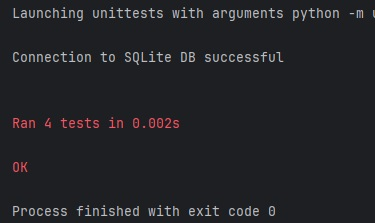
\includegraphics[width=1\linewidth]{images/test2}
	\caption{Результаты выполнения тестов Utils}
	\label{fig:test2}
\end{figure}

\begin{figure}[H]
	\centering
	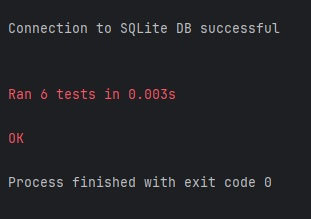
\includegraphics[width=1\linewidth]{images/test3}
	\caption{Результаты выполнения тестов Tables}
	\label{fig:test3}
\end{figure}


\subsection{Интеграционное тестирование программной системы}
Каждое окно приложения представляет уникальный интерфейс, исходя из его функций.  Каждое окно, кроме главного меню, содержит виджет древа.
Древо состоит из:
\begin{itemize}
	\item столбцов с заголовками данных элементов;
	\item данных, внессённых в текущую базу;
	\item полосы прокрутки (появляется, если не все элементы древа помещаются в окно).
\end{itemize}
Главное окно включает в себя кнопки для перехода в другие окна, а также виджет переключателя режимов работы СКУД.
Основное содержимое панели управления меняется в зависимости от выбранной таблицы данных и включает в себя виджеты для изменения, удаления, добавления, поиска и просмотра данных.
Окно проверки доступа включает в себя виджеты для ввода искомых данных, кнопку проверки доступа и виджет переключения режима поиска. Пользователь может просматривать данные различных пассажиров в зависимости от выбранного режима -- <<Пассажир>> или <<Ребёнок>>.

На рисунке ~\ref{fig:example4} представлено главное меню в режиме ЧС.
Режим главного окна пользователь может изменить с помощью переключателя -- от этого будет зависеть дальнейшее поведение системы.
\begin{figure}[H]
	\centering
	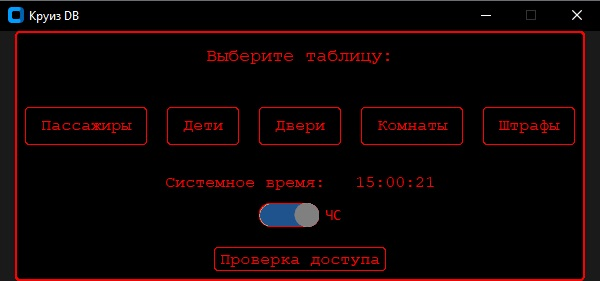
\includegraphics[width=1.0\linewidth]{images/Example4}
	\caption{Главное меню в режиме Чрезвычайной ситуации}
	\label{fig:example4}
\end{figure}

На рисунке ~\ref{fig:example5} представлено окно панели управления данными о штрафах и выбранным штрафом для просмотра детальной информации и последующего изменения. 
Взаимодействовать с элементом можно только тогда, когда он выбран. Его данные отображаются в соответствующих полях для этого вида данных. 
\begin{figure}[H]
	\centering
	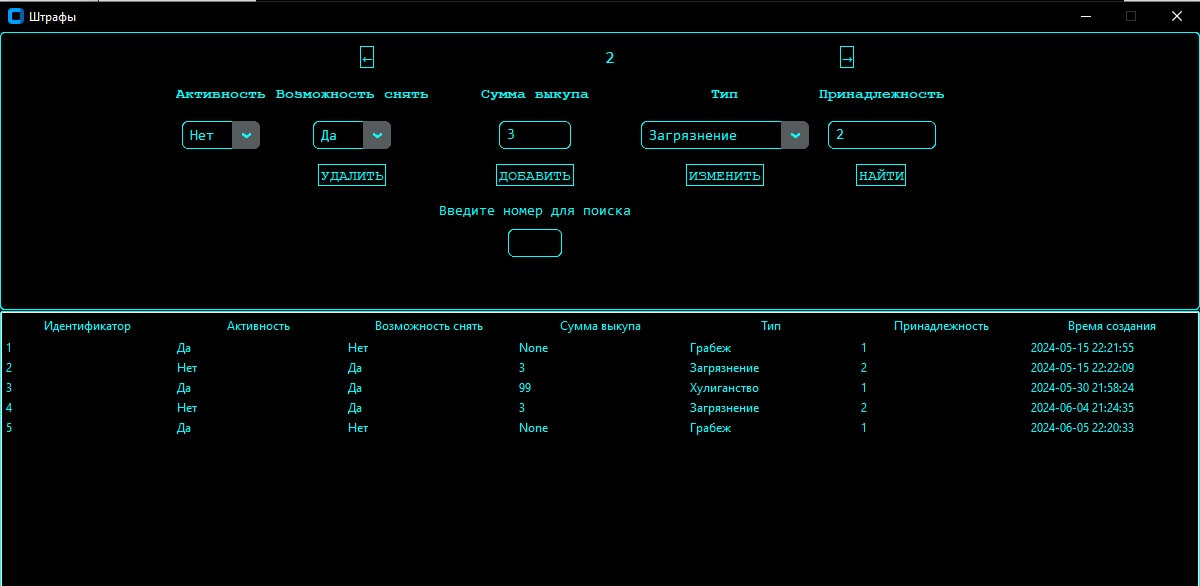
\includegraphics[width=1.0\linewidth]{images/Example5}
	\caption{Панель управления с выбранным элементом}
	\label{fig:example5}
\end{figure}

Менять выбранный элемент пользователь может с помощью виджета \textquotedbl стрелок \textquotedbl, расположенных в верхней части окна, или воспользовавшись опцией поиска, введя в поле \textquotedbl номер для поиска \textquotedbl идентификатор искомого элемента и нажав <<Найти>>. После чего, пользователь получит сообщение о том, был ли найден элемент.
На рисунках  ~\ref{fig:example6} и ~\ref{fig:example7} пользователь видит, что в базе есть данные о пяти штрафах и пытается найти элемент с номером идентификатором 10 и 3 соответственно.
\begin{figure}[H]
	\centering
	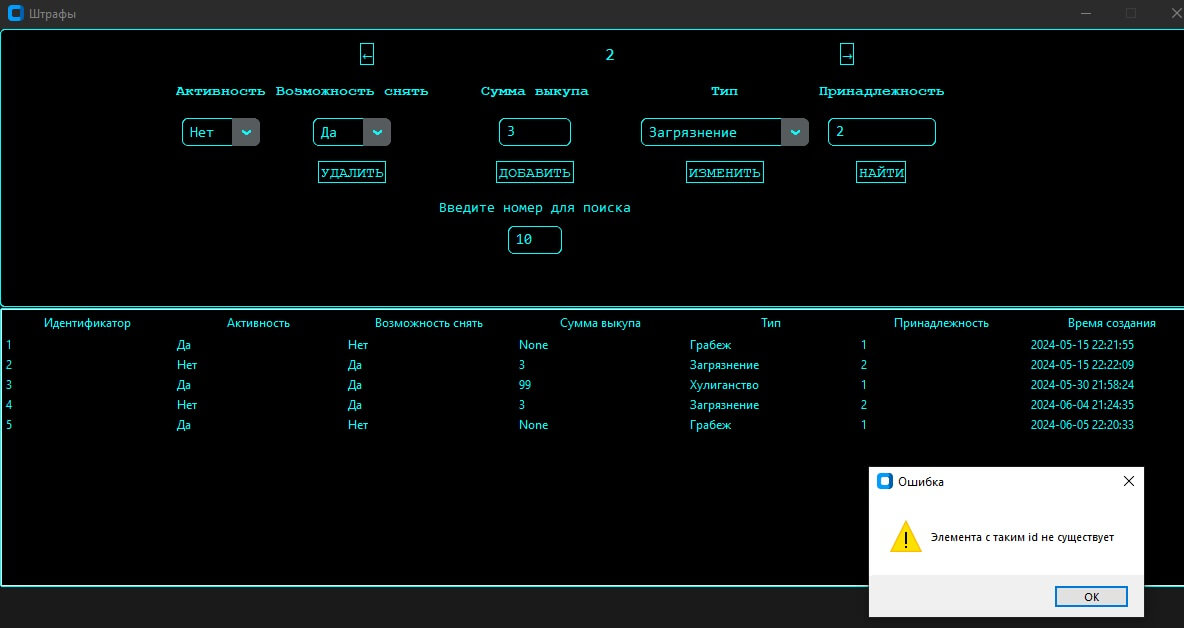
\includegraphics[width=1.0\linewidth]{images/Example6}
	\caption{Поиск несуществующего элемента}
	\label{fig:example6}
\end{figure}

\begin{figure}[H]
	\centering
	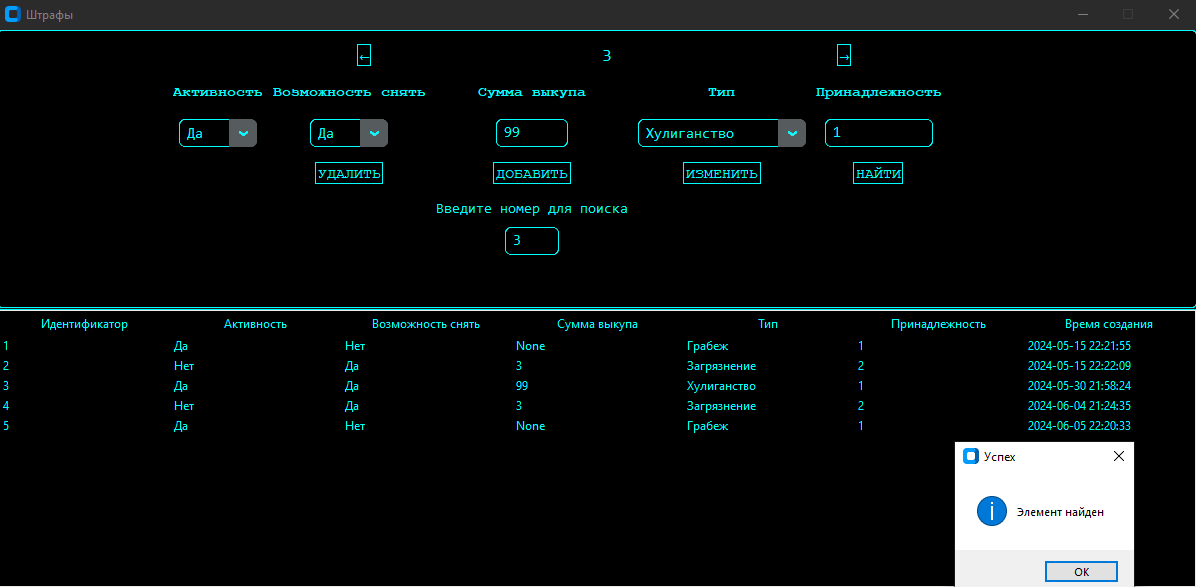
\includegraphics[width=1.0\linewidth]{images/Example7}
	\caption{Поиск существующего элемента}
	\label{fig:example7}
\end{figure}
В случае, когда пользователю нужно зарегистрировать новый штраф, он может добавить новый элемент, посредством заполнения всех обязательных полей и нажатием <<Добавить>>. На рисунке ~\ref{fig:example8} изображен результат добавления нового штрафа в базу.
\begin{figure}[H]
	\centering
	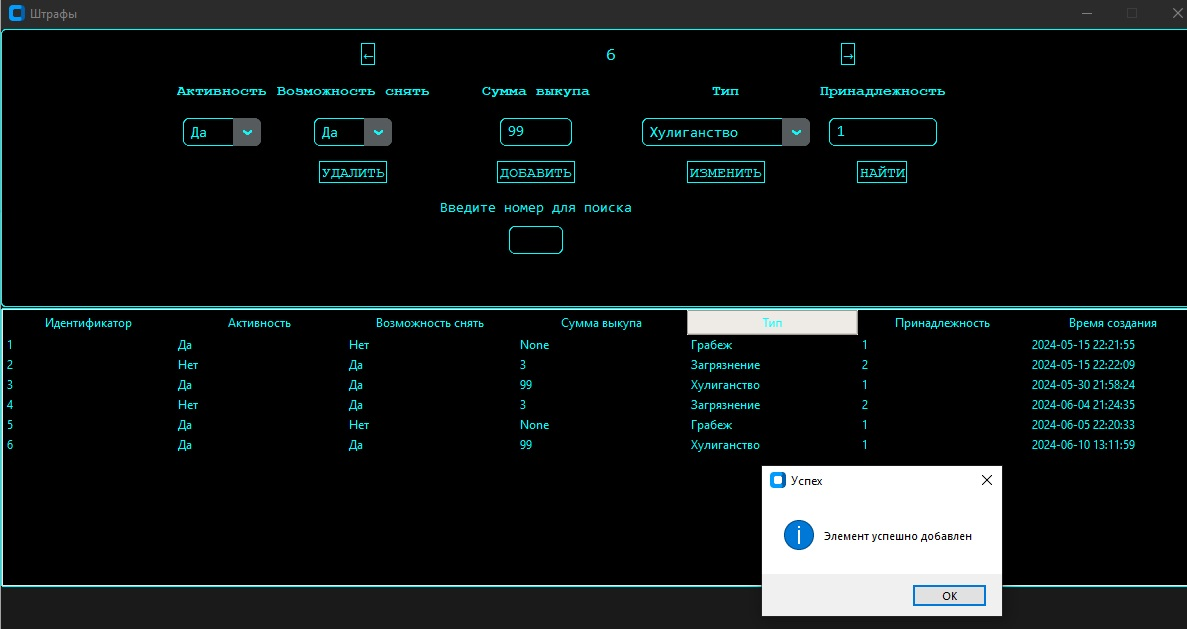
\includegraphics[width=1.0\linewidth]{images/Example8}
	\caption{Добавление нового элемента в панели управления}
	\label{fig:example8}
\end{figure}
Пользователь мог внести и добавить данные об элементе по ошибке. В этом случае он выбирает элемент и удаляет его, посредством клика по кнопке <<Удалить>>.
На рисунке ~\ref{fig:example9} изображён случай удаления недавно добавленного элемента.
\begin{figure}[H]
	\centering
	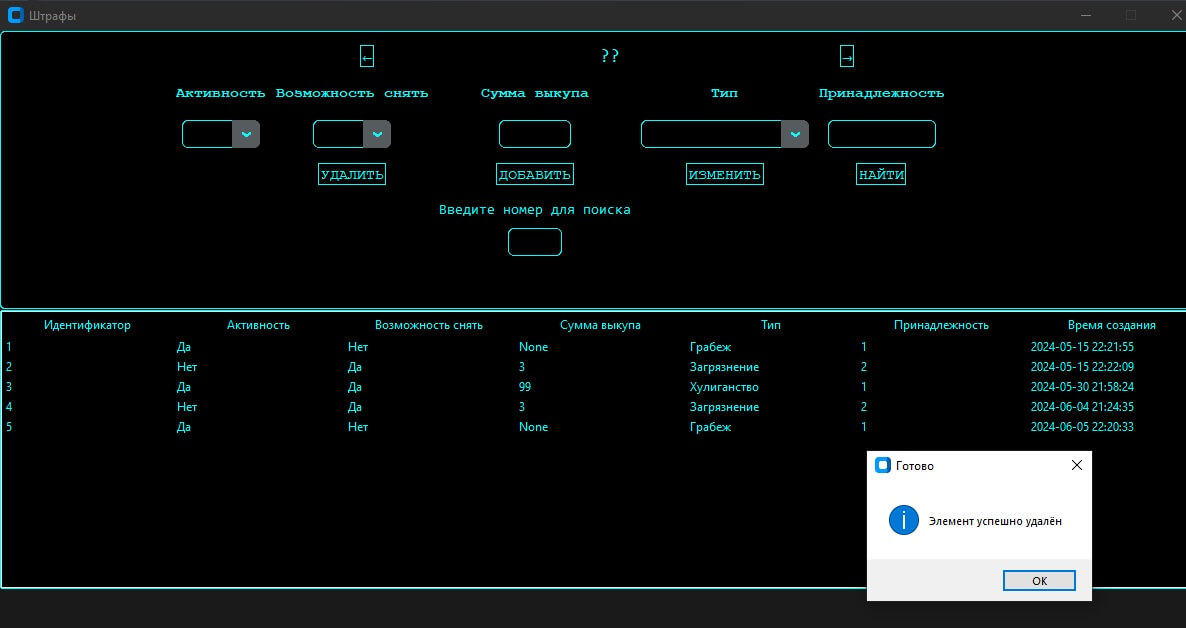
\includegraphics[width=1.0\linewidth]{images/Example9}
	\caption{Удаление данных о штрафе}
	\label{fig:example9}
\end{figure}

На рисунке ~\ref{fig:example10} представлена панель проверки доступа к двери, работающая в режиме <<Ребёнок>> и отражающая в виджете древа данные о доступах детей соответственно. Пользователь может переключить панель в режим <<Пассажир>> для просмотра данных о доступе пассажиров к дверям. При вводе идентификаторов пассажира и двери, и последующем нажатии на <<Проверить доступ>> пользователь получает сообщение о предоставлении доступа, принцип которого был рассмотрен в пункте 3.4 технического проекта.
\begin{figure}[H]
	\centering
	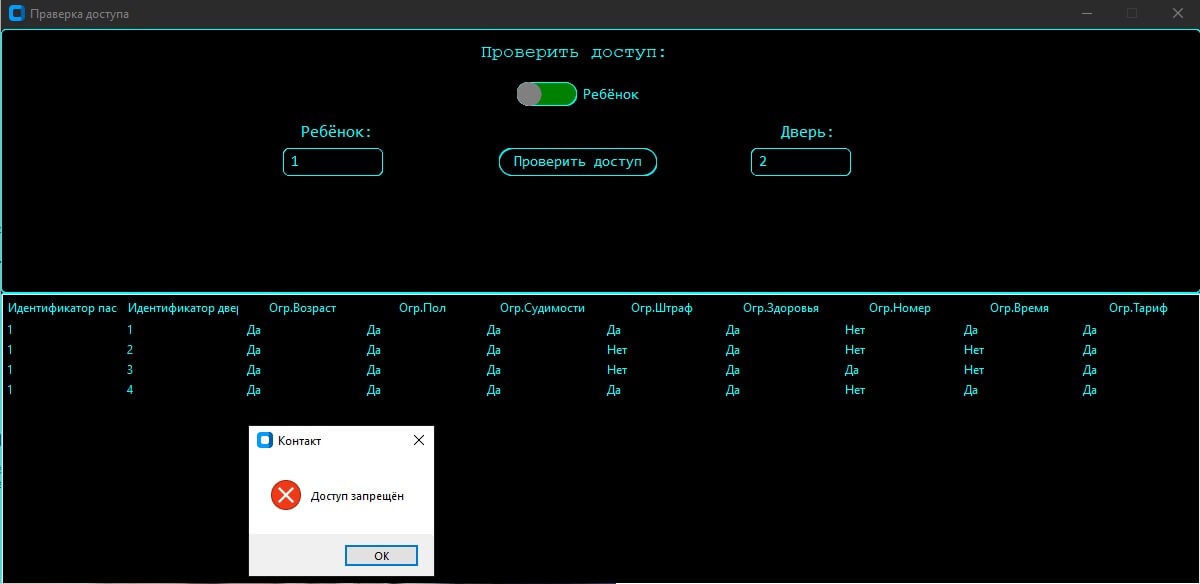
\includegraphics[width=1.0\linewidth]{images/Example10}
	\caption{Проверка доступа к двери}
	\label{fig:example10}
\end{figure}

На рисунке ~\ref{fig:example11} представлена та же панель проверки доступа к двери, однако пользователь зашёл в неё, когда система находилась в режиме ЧС. На этой панели пользователь может совершать те же действия, что и на аналогичной в Штатном режиме, но в режиме ЧС отображается иная таблица о доступе, исходя из правил системы в режиме ЧС, а также интерфейс меняет цвет с голубого на красный, давая понять, что режим системы отличается от штатного.
\begin{figure}[H]
	\centering
	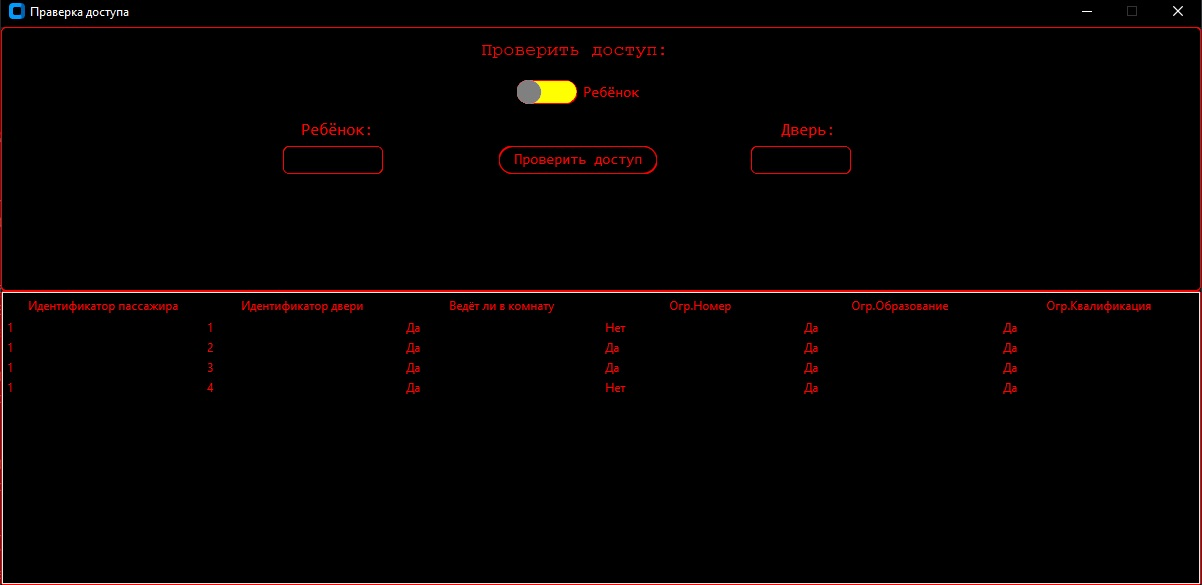
\includegraphics[width=1.0\linewidth]{images/Example11}
	\caption{Альтернативный вид панели}
	\label{fig:example11}
\end{figure}

\newpage